This section provides the reader with additional example aiming to better explain how to adapt such a general hybrid model to specific cases. 

\subsection{Deformable rising droplets}

In a suspension of deformable particles it is known that the drag force is a function of the shapes of the drops.
To take in account such parameter in averaged models one usually use a force correlation function of the Capillary or Morton number. 
However, such models are valid in very specific scenario and flow condition. 
Another way to take in account the particles' deformation or aspect ratio, would be to solve an equation for the mean particle shapes. 
Then, one can create a drag force closure for various particles' aspect ratio. 

\begin{figure}[h!]
    \centering
    \hfill
    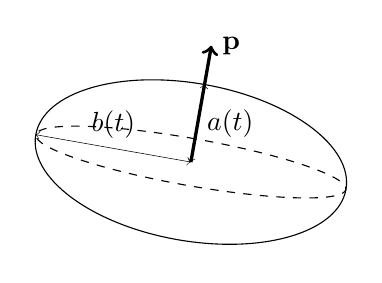
\begin{tikzpicture}[rotate=80]
        \draw(0,0) ellipse (1 cm and 2 cm);
        \draw[dashed](0,0) ellipse (0.3 cm and 2 cm);
        \draw[<->,very thin](0,0) --++ (1,0)node[midway,right]{$a(t)$};
        \draw[->,very thick](0,0) --++ (1.5,0)node[right]{$\textbf{p}$};
        \draw[<->,very thin](0,0) --++ (0,2)node[midway,above]{$b(t)$};
    \end{tikzpicture}
    \hfill
    \caption{Scheme of an  oblate spheroid oriented along the unit vector \textbf{p}.}
    \label{fig:scheme2}
\end{figure}
We consider in this problem an oblate spheroid with a time dependent aspect ratio $\chi = a(t)/b(t)$ oriented along the unit vector \textbf{p}, see \ref{fig:scheme2}.
We consider a mono disperse suspension of droplet with constant mass. 
The objective of this section is to derive constitutive equations to predict the mean orientation, and mean aspect ratio of the droplet. 

\subsubsection{Particle's internal motion}

In the first place we assume a linear homogeneous particle internal motion, such as, 
\begin{equation}
    \textbf{w}_2^0(\textbf{x}_\alpha+ \textbf{r})
    = 
    + \textbf{r} \cdot \textbf{D}_\alpha
    = 
    \bm{\omega}_\alpha \times \textbf{r} 
    + \textbf{r} \cdot \textbf{e}_\alpha
\end{equation}
where $\bm{\omega}_\alpha$ is the angular velocity of the particle, $\textbf{e}_\alpha$ is the mean deformation gradient. 
% Note that the second rank tensor $\textbf{U}_\alpha = \bm{\}$
To respect the mass conservation condition, i.e. $\div \textbf{w}_2^0 =0$, The mean gradient deformation $\textbf{e}_\alpha$ has to respect the conditions : $\textbf{e}_\alpha:\textbf{I}=0$. 
The assumption of linear internal motion is wrong for droplets and bubbles were we are clearly in presence of internal motions. 
However, for now these motions will be discarded. 

\subsubsection{Fundamental properties}

We now compute the mass, moment of mass and moment of momentum of this particle. 
The volume of an ellipsoid reads as, 
\begin{align}
    v_\alpha
    = \frac{4}{3}\pi a b^2
    = \frac{4}{3}\pi \chi  b^3
    \label{eq:volume_def}
\end{align}
Before going further we must say that the two radius $a(t)$ and $b(t)$ are actually dependent since one must preserve the total mass of the particle. 
We recall that we are in the context of mono disperse suspension such that the volume of the particles $v_\alpha$ is actually known, Thus, 
\begin{equation*}
    a(t) 
    = \frac{3 v_\alpha}{4 \pi b^2(t)}
    = \frac{r_0^3}{ b^2(t)}
    \Leftrightarrow
    b^2(t) 
    = \frac{r_0^3}{ a(t)}
\end{equation*}
Where $r_0$ is the radius of the sphere of same volume such as $v_\alpha = \frac{4}{3}\pi r_0^3$. 
Also, it might be useful to compute the relation between the derivative of the radius,  
\begin{equation*}
    \ddt v_\alpha 
    % = \ddt \frac{4}{3}\pi a b^2
    = \frac{4}{3}\pi \dot{a}(t) b^2(t)
    + \frac{8}{3} \pi {a}(t) b(t) \dot{b}(t)
    = 0 
    \Leftrightarrow
     \dot{a}(t)
    =  
    - 2 \frac{a(t)}{b(t)}  \dot{b}(t)
    % \Leftrightarrow
\end{equation*}
Which means that the derivative of both radius are related to twice the aspect ratio. 

The second moment of mass is somewhat more complicated to compute, we have, 
\begin{align*}
    \mathcal{M}_{\alpha,ij}
    = \int r_ir_j dxdydz
\end{align*}
At this stage we would like to compute the integral in spherical coordinate, thus we introduce the change of variables, 
\begin{align*}
    x' = x/a 
    && y' = y/b 
    && z' = z/b 
\end{align*}
By assuming that the spheroid is aligned with the $z$ axis and centered at the origin we get, 
\begin{align*}
    \mathcal{M}_{\alpha,zz}
    = a(t)^3 b(t)^2 \int z'z' dx'dy'dz'
\end{align*}
switching in spherical coordinate yields 
\begin{align*}
    \mathcal{M}_{\alpha,zz}
    = a(t)^3 b(t)^2 \int_0^1 \int_0^{2\pi}\int_0^\pi r^4 \cos^2\phi \sin\phi d\phi d\theta dr
    = a(t)^3 b(t)^2 \frac{1}{5}\frac{4}{3} \pi
    = v_\alpha \frac{a^2(t)}{5}\\
    \mathcal{M}_{\alpha,xx}
    = a(t) b(t)^4 \int_0^1 \int_0^{2\pi}\int_0^\pi r^4 \sin^3\phi\cos^2\theta d\phi d\theta dr
    = a(t) b(t)^4
    \frac{1}{5}
     \frac{4}{3}
     \pi
     =v_\alpha \frac{b^2(t)}{5}
\end{align*}
In a more general manner one can define the tensor $\mathcal{M}_\alpha$ in the laboratory reference frame using the orientation tensor \textbf{p}, such that, 
\begin{equation}
    5 \frac{\mathcal{M}_{\alpha,ij}}{v_\alpha}
    = p_i p_j 
    a^2(t) 
    + (\delta_{ij} - p_ip_j) b^2(t)
    = H_{ij}^{-1}
    \label{eq:M_alpha_def}
\end{equation} 
In light of \ref{eq:M_alpha_def}we reduced the description of any particle in our flow to four parameters, the 3 components of \textbf{p}, and the radius $a(t)$. 


Now let's compute the first moment of momentum $\mathcal{P}_\alpha$, it reads, 
\begin{align*}
    \mathcal{P}_{\alpha,ij}
    = \int r_i w_{2,j}^0 d\Omega
    = D_{\alpha,jk} \mathcal{M}_{\alpha,ki}
    = \epsilon_{jkl} \omega_{\alpha,k} \mathcal{M}_{\alpha,il}
    +  e_{\alpha,jk} \mathcal{M}_{\alpha,ik}
\end{align*}
Taking the double contracted product with $\epsilon_{mij}$ of the moment of momentum yield the angular momentum equation, 
\begin{align*}
    \mu_{\alpha,m}
    = \epsilon_{mij}\mathcal{P}_{\alpha,ij}
    = \epsilon_{jmi} \epsilon_{jkl} \omega_{\alpha,k} \int r_i r_l  d\Omega
    +  \epsilon_{mij} e_{\alpha,jk} \int r_i r_k  d\Omega\\
    = (\delta_{mk}\mathcal{M}_{\alpha,ll} - \mathcal{M}_{\alpha,mk}) \omega_{\alpha,k}
    +  \epsilon_{mij} e_{\alpha,jk} \int r_i r_k  d\Omega\\
    = \mathcal{I}_{\alpha,mk} \omega_{\alpha,k}
    +  \epsilon_{mij} e_{\alpha,jk} \mathcal{M}_{\alpha,ik}\\
\end{align*}
The second contribution of the angular momentum would vanish if the particles where spherical. 
Lastly, the symmetric part of the moment of momentum reads, 
\begin{align*}
    2\mathcal{S}_{\alpha,ij}
    = \epsilon_{jkl} \omega_{\alpha,k} \mathcal{M}_{\alpha,il}
    + \epsilon_{ikl} \omega_{\alpha,k} \mathcal{M}_{\alpha,jl}
    +  e_{\alpha,jk} \mathcal{M}_{\alpha,ik}
    +  e_{\alpha,ik}  \mathcal{M}_{\alpha,jk}
\end{align*}

\subsubsection*{Evolution equation of a single particle shpae.}

We first start by the kinetic equations.  
In view of the previous expression the evolution equation of the momentum tensor is,  
\begin{equation*}
    \ddt \mathcal{M}_{\alpha,ij}
    + \epsilon_{jlk} \omega_{\alpha,k} \mathcal{M}_{\alpha,il}
    - \epsilon_{ikl} \omega_{\alpha,k} \mathcal{M}_{\alpha,jl}
     =  e_{\alpha,jk} \mathcal{M}_{\alpha,ik}
     +  e_{\alpha,ik}  \mathcal{M}_{\alpha,jk}
     \label{eq:dt_M_alpha_bis}
\end{equation*}
On the left-hands-side of \ref{eq:dt_M_alpha_bis} we clearly identify the Jaumann derivative rotating with the vorticity.
To close this equation one may relate the mean ambient flow variables to the particles angular rotation and stretching rate. 
This however this is only possible considering pure stokes flow.

\subsubsection*{Equation for the bulk stress}

The equivalent stress can be formulated as, 
\begin{equation*}
    \bm{\sigma}
    = 
    \phi_1 \bm{\sigma}_1
    + \phi_2 \bm{\sigma}_2
    + \phi_I \bm{\sigma}_I
    \label{eq:sigma_def}
\end{equation*}
The particle phase stress can be reduced to its first moment, $\phi_2 \bm{\sigma_2} = \pOavg{\bm{\sigma}_2^0}$ and thus, 
\begin{equation*}
    \phi_2 \bm{\sigma}_2 
    = - \phi_2 p_2
    + \phi_2 \mu_2 \textbf{e}_p 
\end{equation*}
Using the following expression for $\phi_1 \bm{\sigma}_1 = - \phi_1 p_1 + \mu_1 \phi_1 \textbf{e}_1 =  - \phi_1 p_1 + \mu_1 \textbf{e} - \mu_1 \phi_2 \textbf{e}_2$.
Likewise since we considered a constant strain within the particle we can write $\phi_2\textbf{e}_2 = \phi_2 \textbf{e}_p$ in homogeneous medium.   
The previous expression of the averaged stress yields, 
\begin{equation*}
    \bm{\sigma}
    = 
    - p 
    + \mu_1 \textbf{e} 
    + (\mu_2 - \mu_1) \phi_2 \textbf{e}_2
    + \phi_I \bm{\sigma}_I
    \label{eq:sigma_def}
\end{equation*}
In the above stress equation $\bm{\sigma}_I$ is unknown and must be closed. 
While the others parameters can be easily linked to our problem variable. 

We recall that in homogeneous flows, $\phi_I \bm{\sigma}_I = \gamma\pSavg{\textbf{I}-\textbf{nn}}$. 
Therefore, to close this term one must compute the curvature of the particles. 
The first moment of surface tension stress can be computed analytically following \citep{nadim1996concise} for the curvature computation.
In this context an equation describing the droplets surface can be found in the reference frame of the droplets, namely, 
\begin{equation}
    \mathscr{F}
    = \textbf{r}\cdot \textbf{H}\cdot \textbf{r} - 1 = 0 
    \label{eq:F_def}
\end{equation}
where \textbf{H} is a symmetric traceless tensor such that $\textbf{H} = \textbf{pp}/a^2(t) + (\textbf{I}- \textbf{pp})/b^2(t)$. 
This analytical expression will enable us to compute the curvature of each particle.  
Let $\mathscr{F}(\textbf{x},t) = 0$ be the equality representing the ellipsoidal shape of the particle. 
First, the normal pointing in the direction of positive $\mathscr{F}$ at the interface, can be computed as, 
\begin{equation*}
    \textbf{n} = \frac{\grad \mathscr{F}}{(\grad \mathscr{F}\cdot \grad \mathscr{F})^{1/2}} \;\;\text{ on }\;\; \mathscr{F} = 0.  
\end{equation*}
It follows that the local surface stress is, 
\begin{equation*}
    \bm{\sigma}_I^0 =
    \gamma \left[\textbf{I} - \frac{\grad \mathscr{F} \grad \mathscr{F}}{\grad \mathscr{F}\cdot \grad \mathscr{F}}\right] \;\;\text{ on }\;\; \mathscr{F} = 0.  
\end{equation*}
Noticing that $\grad \mathscr{F} = 2\textbf{H}\cdot \textbf{r}$ one obtain, 
\begin{equation*}
    \bm{\sigma}_I^0 =\gamma\left[
    \textbf{I} - \frac{ \textbf{HH} :  \textbf{rr}}{ (\textbf{H}\cdot  \textbf{H}\cdot \textbf{rr})} \right]
\end{equation*}
In indices notation,  
\begin{equation*}
    \sigma_{I,ij}^0 =\gamma\left[
    \delta_{ij} - \frac{ H_{ik} H_{jl} :  r_kr_l}{  H_{ab}  H_{ac} r_br_c} \right]
\end{equation*}
Integrating this over a surface will eventually leads to an elliptic integral due to the elliptical surface. 
\subsubsection*{Equation for the particles strain}

Additionally, using the first moment of momentum expression one can obtain an other expression for the particles internal stress, 
\begin{equation}
    \intS{ (\bm{\sigma}_I)_{ik}}
    +\intO{ (\bm{\sigma}_2^0)_{ik}}
    = 
    \intO{ \rho_2 
    (\textbf{w}_2^0\textbf{w}_2^0  )_{ik}
    }
    -\ddt \intO{ r_i (\textbf{u}^0_2)_k }
    +\intS{ 
     r_i (\bm{\sigma}_1^0 \cdot \textbf{n}_2)_{k}
    }
\end{equation}
\subsection{Equation for the particle angular momentum}
\begin{equation*}
    \ddt \mu_p = t_p
\end{equation*}